\clearpage
\section{Spurious Outputs}
\label{sec:spurious-outputs}
\raggedbottom% short text pages end short instead of stretching the gaps (the figure follows on its own)
% numbers: sections/sec_spur_numbers.tex, loaded in the Key Specifications section (it is quoted there first)

Besides the signal you ask it to transmit, every real transmitter also puts out small, unwanted tones at other
frequencies. These are called spurious outputs, or ``spurs''. A spur carries no information; it is simply RF energy
at a frequency you did not ask for. Spurs matter for two reasons: they can interfere with other radios (including
other Pi-Radio units) that are listening at the spur's frequency, and they count against the spectrum-emission
limits that apply whenever a transmitter is connected to an antenna. This section lists the spurs we have
characterized on this unit.

\subsection{TX-side 2×LO Spur}
\label{sec:spur-tx-2lo}

\textbf{What it is.} The LO is a strong signal inside the unit, and every real oscillator and amplifier produces
harmonics of its signal. Some of the second harmonic of
the LO, at exactly twice the LO frequency (``2×LO''), appears at the ``TX-side FR3 RF Out'' connector as a spur.
Its frequency depends only on the LO, so to find it, first work out the LO from your FR1 and FR3 settings: for the
upper sideband, LO~=~FR3~$-$~FR1; for the lower sideband, LO~=~FR3~+~FR1. For example, FR1~=~1\,GHz and
FR3~=~9\,GHz in the upper sideband gives LO~=~8\,GHz, so the 2×LO spur is at 16\,GHz. The spur is always well
away from the wanted signal, but it can land inside the 6--24\,GHz FR3 band, where another unit or receiver may be
working.

\textbf{How we measured it.} At each of \twoLoLoCount{} LO frequencies from \twoLoLoMin{} to \twoLoLoMax\,GHz, in 100\,MHz steps, with nothing connected to the ``TX-side FR1 IF In'' port, the LO leakage was first nulled with the reference filter, exactly as in the calibration of Section~\ref{sec:lo-suppression}. The power at 2×LO was then read at the ``TX-side FR3 RF Out'' connector (cable loss removed) in \emph{every} filter setting that can be in use at that LO frequency --- every setting the optimal-filter rule can select for any FR1 from 0.7 to 4.0\,GHz, in either sideband --- \twoLoReadCount{} readings in all. The unit was measured hot, as the worst case (no fan, LMX2820 die at \twoLoMinC--\twoLoMaxC\textdegree C), with \lmxDriveRule.

\textbf{What you get.} Figure~\ref{fig:spur-1} shows the result: at each LO frequency, the median over all the filter settings and the range from the lowest to the highest. The median of all \twoLoReadCount{} readings is \twoLoMedian\,dBm. The filter setting makes a large difference, often 20\,dB or more at the same LO frequency. The highest reading is \twoLoMax\,dBm (LO~=~\twoLoMaxLo\,GHz, filter \twoLoMaxFilter); only \twoLoAboveTwenty{} of the \twoLoReadCount{} readings are above $-$20\,dBm, all of them at LO frequencies from \twoLoAboveLoMin{} to \twoLoAboveLoMax\,GHz. The level also changes quickly from one LO frequency to the next, so read the figure as an envelope rather than as an exact value at any one frequency.

\textbf{What it does not depend on.} The spur level does not depend on the signal you transmit: with a 1\,GHz
input tone switched on after the LO was nulled, the 2×LO spur changed by less than 1\,dB at \spurToneWithinOne{}
of \spurToneCount{} LO frequencies (median change \spurToneMedianDiff\,dB). It also does not depend on how well the
LO leakage is nulled, as long as the LO leakage itself stays below about $-$10\,dBm. Above that, the spur grows
quickly: with the LO leakage deliberately raised to +10\,dBm, the 2×LO spur rose to between \spurAmpLow{} and
\spurAmpHigh\,dBm, and with the LO leakage left uncorrected (I\_V~=~Q\_V~=~0\,V, LO leakage up to
+\spurZeroBiasLoMax\,dBm) it reached \spurZeroBiasWorst\,dBm. Keeping the LO-leakage calibration of
Section~\ref{sec:lo-suppression} applied therefore also keeps the 2×LO spur at the levels of
Figure~\ref{fig:spur-1}.

\textbf{Variation between units.} These results are from one unit. We expect differences of a few dB from one unit to the next, and expect the 2×LO spur to stay below $-$20\,dBm on any unit for a vast majority of configurations.

\textbf{Measurement limit.} For LO frequencies above \spurLoLimit\,GHz, the 2×LO spur lies above
\spurTwoLoLimit\,GHz, which is the rated limit of the unit's SMA connectors and of the test equipment we used; it
was not measured there.

\textbf{Practical advice.} For cabled measurements, where your receiver or analyzer is tuned to the FR3 frequency,
the 2×LO spur usually needs no action. When you transmit over the air with a wideband antenna, or share the band
with other receivers that may be tuned near 2×LO, add an external low-pass or band-pass filter after the
``TX-side FR3 RF Out'' connector that passes your FR3 frequency and blocks 2×LO.

\begin{center}
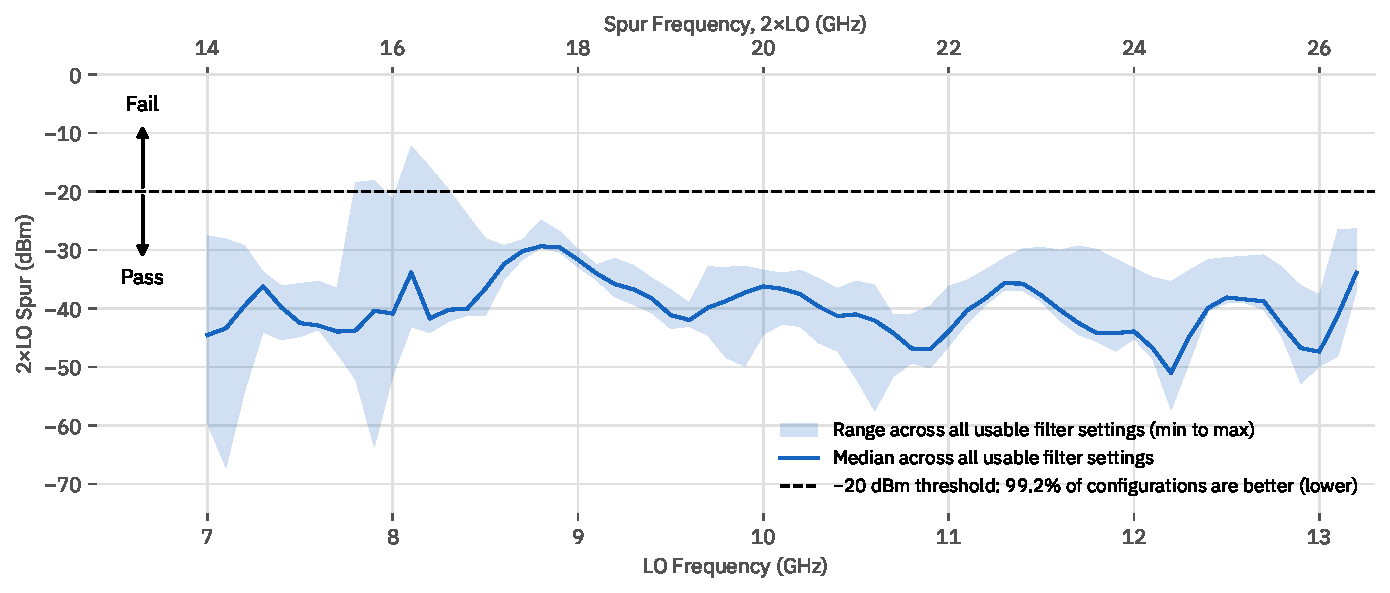
\includegraphics[width=\linewidth]{images/sec_spur_2lo_all_filters.pdf}
\captionof{figure}{TX-side 2×LO spur at the ``TX-side FR3 RF Out'' connector at \twoLoLoCount{} LO frequencies (\twoLoLoMin--\twoLoLoMax\,GHz in 100\,MHz steps; top axis: the spur frequency, 2×LO). At each LO frequency the LO leakage was nulled with the reference filter, and the 2×LO was read in every filter setting usable at that LO frequency, with no input signal. The line is the median across those settings, and the shaded band spans the lowest to the highest. The dashed line marks $-$20\,dBm.}\label{fig:spur-1}
\end{center}
\subsection{RX-side LO and 2×LO Leakage}
\label{sec:spur-rx-lo}

\textbf{Why it matters.} The RX side is meant only to receive, but the LO is running inside the unit the whole time,
and a little of it, along with its second harmonic (2×LO), leaks backwards out of the ``RX-side FR3 RF In''
connector. With a cable to a signal generator or another unit this does no harm. With an antenna connected, however,
whatever leaks out of that connector is radiated: the unit transmits a weak tone at the LO frequency, and another at
2×LO, even while it is only receiving. Those tones can interfere with other receivers nearby (including other
Pi-Radio units in the same experiment), and they count against the emission limits that apply to anything connected
to an antenna.

\textbf{How we measured it.} At each LO frequency, the unit was set up as it would be in normal use: \lmxDriveRule{} (set from the LO frequency); the TX side with its stored LO-leakage calibration applied and its optimal filter engaged (with the ``TX-side FR3 RF Out'' connector terminated in 50\,$\Omega$); and the RX filter in its ``optimal'' state for FR3~=~LO~+~1\,GHz. Nothing else was connected. A spectrum analyzer on the ``RX-side FR3 RF In'' connector (cable loss removed) read the power at the LO frequency and at 2×LO. The LO leakage was measured at \rxLeakLoCount{} LO frequencies from \rxLeakLoMin{} to \rxLeakLoTop\,GHz in 100\,MHz steps; 2×LO was measured at the \rxLeakTwoLoCount{} LO frequencies up to \rxLeakLoFineMax\,GHz, where 2×LO stays within \spurTwoLoLimit\,GHz. The unit was measured hot: no fan, LMX2820 die at \rxLeakLmxMinC--\rxLeakLmxMaxC\textdegree C.

\textbf{What you get.} Figure~\ref{fig:spur-2} shows the LO leakage, and Figure~\ref{fig:spur-3} the 2×LO leakage.
The LO leakage out of the ``RX-side FR3 RF In''
connector has a median of \rxLeakLoMedian\,dBm and reaches at most \rxLeakLoMax\,dBm (at LO~=~\rxLeakLoMaxAt\,GHz).
The 2×LO leakage has a median of \rxLeakTwoLoMedian\,dBm and reaches at most \rxLeakTwoLoMax\,dBm (at
LO~=~\rxLeakTwoLoMaxAt\,GHz). The LO leakage is lowest at the bottom of the LO range (\rxLeakLoBest\,dBm at
LO~=~\rxLeakLoBestAt\,GHz) and highest in the middle of it, around LO~=~\rxLeakLoMaxAt\,GHz. As for the TX-side spur,
these results are from one unit, and we expect differences of a few dB from one unit to the next.

\textbf{It does not depend on the TX-side calibration.} At \rxLeakOffsetCount{} of the LO frequencies
(\rxLeakOffsetLos\,GHz) we repeated the reading with the TX LO-leakage bias deliberately moved \rxLeakOffsetMv\,mV
away from its null, which raises the TX-side LO leakage by tens of dB. The leakage out of the ``RX-side FR3 RF In''
connector changed by at most \rxLeakOffsetMaxChange\,dB. So the RX-side leakage does not depend on how well the TX side
is calibrated, or on the TX side's calibration drifting with time and temperature.

\textbf{Measurement limit.} For LO frequencies above \spurLoLimit\,GHz, 2×LO lies above \spurTwoLoLimit\,GHz, the
rated limit of the unit's SMA connectors and of our test equipment, and was not measured there.

\textbf{Practical advice.} If you receive through an antenna and the leakage matters for your experiment, add a
band-pass filter between the antenna and the ``RX-side FR3 RF In'' connector that passes your FR3 frequency and
rejects the LO. Because the LO is exactly FR1 away from FR3, choosing a larger FR1 moves the LO further from your
signal and makes such a filter easier to build.

\noindent\begin{minipage}{\linewidth}
\centering
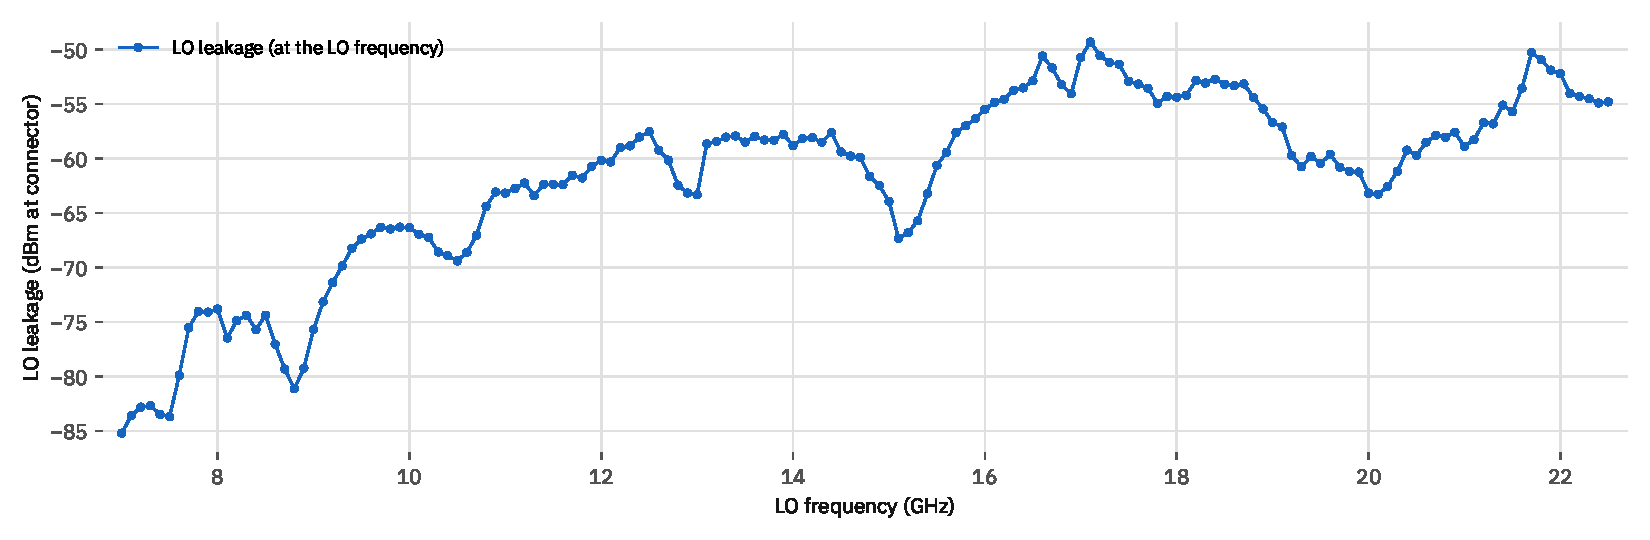
\includegraphics[width=\linewidth]{images/sec_spur_fig2.pdf}
\captionof{figure}{LO leakage at the ``RX-side FR3 RF In'' connector against LO frequency. LMX2820 drive rule; TX side in normal use (stored LO-leakage calibration, optimal filter), ``TX-side FR3 RF Out'' terminated in 50\,$\Omega$; RX filter optimal for FR3~=~LO~+~1\,GHz; nothing else connected.}\label{fig:spur-2}
\end{minipage}

\bigskip
\noindent\begin{minipage}{\linewidth}
\centering
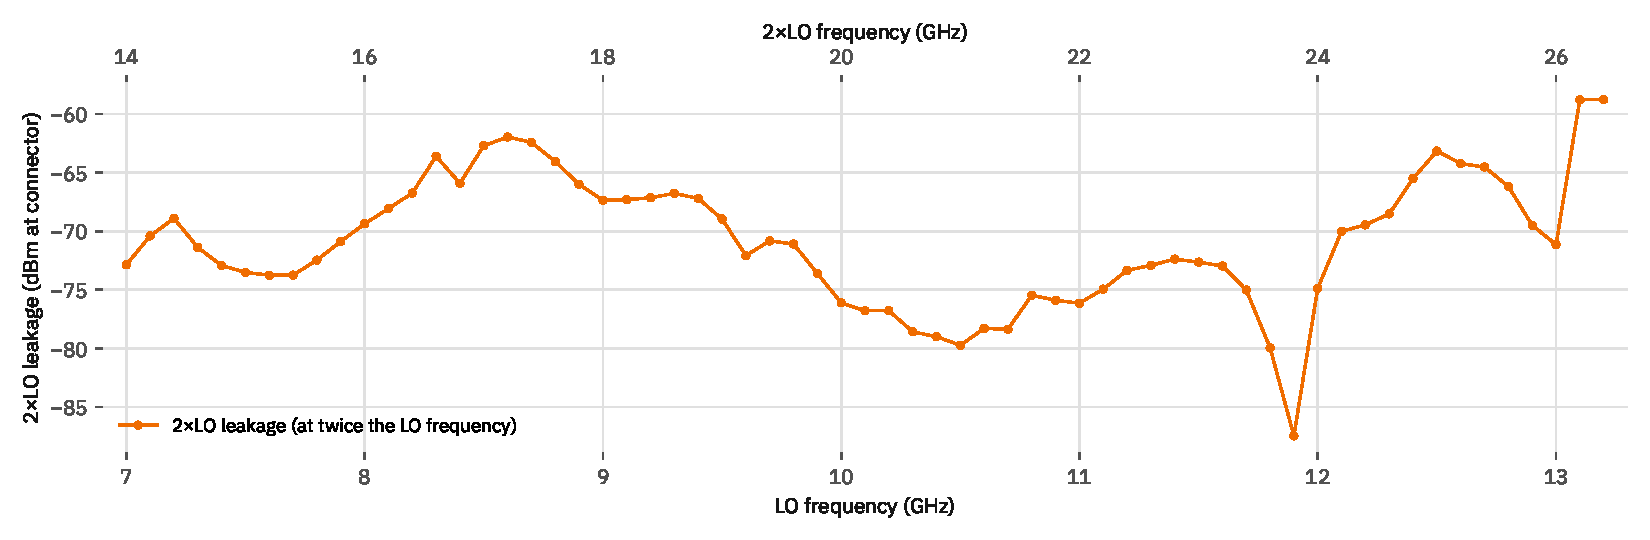
\includegraphics[width=\linewidth]{images/sec_spur_fig3.pdf}
\captionof{figure}{2×LO leakage at the ``RX-side FR3 RF In'' connector against LO frequency (top axis: the 2×LO frequency), in the same set-up as Figure~\ref{fig:spur-2}. Measured for LO up to \rxLeakLoFineMax\,GHz: above \spurLoLimit\,GHz, 2×LO would exceed \spurTwoLoLimit\,GHz, the limit of the connectors and test equipment.}\label{fig:spur-3}
\end{minipage}

\flushbottom
